\chapter{Autenticazione dell'utente}
Il processo di autenticazione è uno dei primi metodi utilizzabili per proteggersi da attacchi informatici. Consiste nel verificare l'identità dell'utente, ovvero che sia chi dice di essere. 
Questo è importante per:
\begin{itemize}
    \item Garantire la proprietà di authentication -> se ho l'identità di un utente verificata, gli posso associare i permessi per lui previsti all'interno del sistema;
    \item Garantire la proprietà di accountability -> posso determinare chi ha effettuato determinate azioni all'interno del sistema (mantengo log sull'utente).
\end{itemize}

Ci sono tre modi principali per verificare l'identità di un utente, che possono essere usati singolarmente o in combinazione:
\begin{itemize}
    \item Tramite un segreto che l'utente possiede;
    \item Tramite qualcosa che l'utente possiede;
    \item Tramite qualcosa che l'utente è.
\end{itemize}

\paragraph{Autenticazione con sistemi biometrici} Come per le smart card, è necessario uno scanner della caratteristica biometrica che l'utente usa per autenticarsi. 
Le caratteristiche utilizzabili per autenticarsi devono essere:
\begin{itemize}
    \item Universali -> comuni a tutti gli individui;
    \item Distintive -> ogni persona dovrebbe avere differenze notabili in quella caratteristica;
    \item Permanenza -> la caratteristica non dovrebbe cambiare notevolmente nel tempo;
    \item Collezionabili -> la caratteristica dovrebbe essere effettivamente determinabile e quantificabile.
\end{itemize}

\noindent La caratteristica viene quantificata tramite lo scanner e salvata. Al momento dell'autenticazione, il sistema confronterà il dato precedentemente salvato con quello quantificato al momento: se la differenza è limitata, l'utente viene autenticato.

\noindent Esempi: firma, impronta digitale, retina, voce, volto, ...

\noindent Problemi: gli algoritmi usati possono generare falsi positivi (autorizzo un utente che non sarbbe autorizzato) e falsi negativi (non autorizzo un utente legittimo); a seconda della caratteristica scelta, un attaccante potrebbe facilmente rubarla (es: impronta digitale); l'utente potrebbe non voler farsi scannerizzare una determinata caratteristica. 

\section{Autenticazione con password}
Si tratta di sistemi semplici e poco costosi da implementare, ma molto vulnerabili ad attacchi, principalmente in quanto richiedono agli utenti uno sforzo cognitivo superiore a quello che sono in grado di effettuare. 

Uno dei problemi è che gli utenti utilizzano le stesse password sia in ambito domestico e lavorativo.

\subsection{Attacchi alle password}
Esistono diversi attacchi che permettono agli attaccanti di ottenere le password delle vittime:
\begin{itemize}
    \item Offline attacks: hanno l'obiettivo di accedere al **password file** salvato sul server di autenticazione in cui sono contenute tutte le password degli utenti;
    \item Online attacks: possono essere attivi o passivi. Richiedono che gli attaccanti interagiscano con l'obiettivo dell'attacco (es: servizio di cui voglio ottenere la password per accedere, account sul pc dell'organizzazione). Negli attacchi attivi, l'attaccante prova diverse password per trovare quella corretta, mentre in quelli passivi utilizza altri metodi, come l'intercettazione del traffico dell'utente;
    \item Non technical attacks: utilizzano tecniche di ingegneria sociale per ottenere le credenziali.
\end{itemize}

\noindent Tra le tecniche di attacco ci sono:
\begin{itemize}
    \item Attacchi di brute force;
    \item Attacchi con key logger;
    \item Attacchi con mail di phishing;
\end{itemize}

\subsection{Attacchi offline}
Dove sono memorizzate le password?
\begin{itemize}
    \item In Windows il password file è accessibile in due modi: 
    	\begin{itemize}
    	    \item In C:$\backslash$Windows$\backslash$System32$\backslash$config nel file SAM;
    	    \item Nei registri di Windows sotto HKEY\_LOCAL\_MACHINE -> SAM -> SAM. 
    	\end{itemize}
     \noindent Solitamente l'accesso al file è garantito solo ad account amministratore o system.
    \item In Linux ci sono due file usati per salvare la password:
    	\begin{itemize}
    	    \item $\backslash$etc$\backslash$passwd contiene gli user di tutti gli utenti collegati alla macchina;
        	\item $\backslash$etc$\backslash$shadow contiene gli hash delle password memorizzate nel password file.
    	\end{itemize}
\end{itemize}

\noindent Generalmente un password file memorizza quattro parametri per le password (figura \ref{fig:7-1}):
\begin{itemize}
    \item Utente;
    \item SID;
    \item Due Hash.
\end{itemize}

\begin{figure}
    \centering
    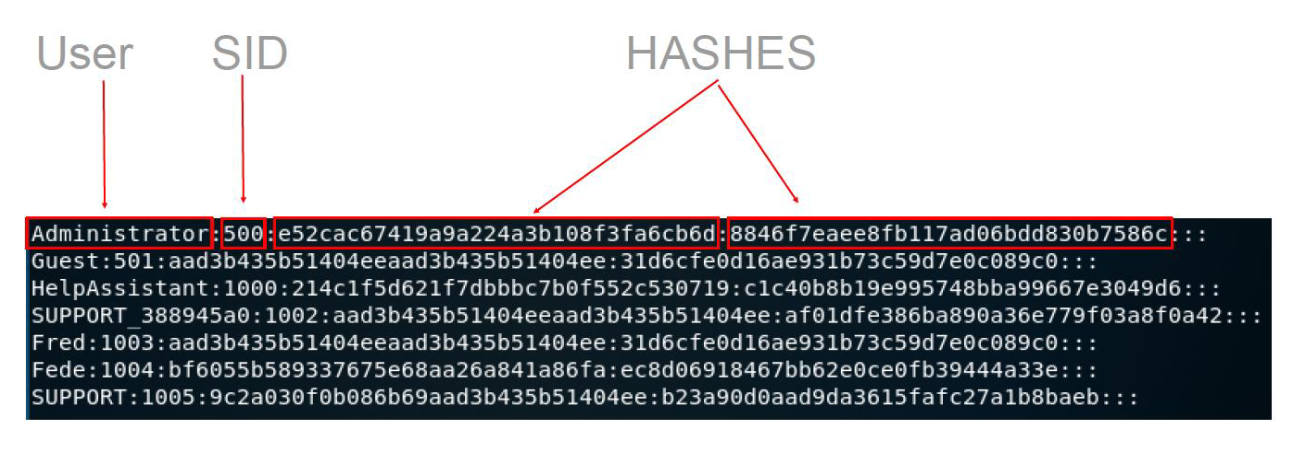
\includegraphics[width=0.7\textwidth]{images/7-1.png}
    \caption{Esempio di password file.}
    \label{fig:7-1}
\end{figure}

\noindent Salva quindi il nome dell'utente, un SID associato a tale nome e due hash della password, create tramite due algoritmi differenti (figura \ref{fig:7-2}):
\begin{itemize}
    \item LM: usato da sistemi Windows fino alla versione XP. Crea hash a 128 bit ma utilizza un character set set di 142 caratteri e accetta password si max 14 caratteri. Divide la password in due sottostringhe di 7 caratteri e non è case sensitive (genera lo stesso hash se le due password sono uguali ma una con caratteri maiuscoli e una minuscoli);
    \item NTLM: introdotto successivamente e più sicuro. Crea hash a 128 bit ma utilizza tutti i caratteri ASCII e accetta password di max 256 caratteri. Non divide la password ed è case sensitive.
\end{itemize}

\begin{figure}
    \centering
    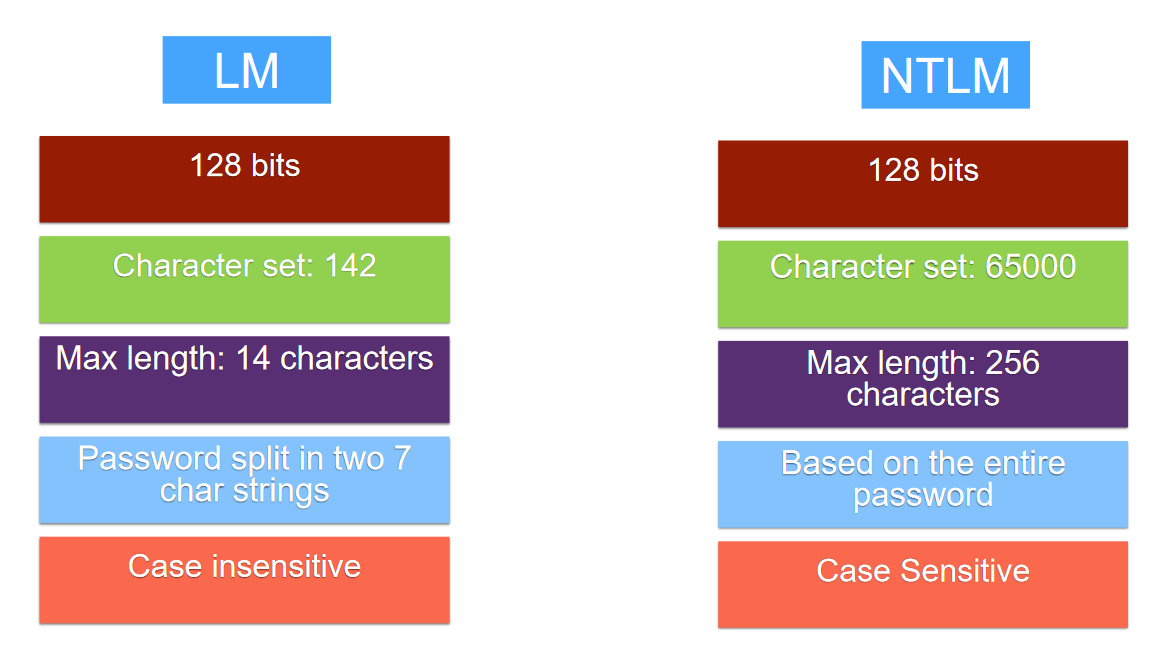
\includegraphics[width=0.6\textwidth]{images/7-2.png}
    \caption{Algoritmo LM e nTLM.}
    \label{fig:7-2}
\end{figure}

\noindent Per motivi di compatibilità, nelle versioni più recenti di Windows, sono presenti entrambi gli hash. 

\paragraph{Algorimo LM}
\begin{itemize}
    \item Memorizza password di max 14 caratteri;
    \item Converte tutti i caratteri a MAIUSCOLI;
    \item Filla gli spazi vuoti della passwword fino a raggiungere 14 caratteri;
    \item Divide la password in due sottostringhe di 7 caratteri;
    \item Cifra separatamente le due sottostringhe;
    \item Combina i due risultati.
\end{itemize}

 \paragraph{Principali attacchi offline}
 I principali attacchi offline sono tre: 
 \begin{enumerate}
     \item Attacchi di forza bruta (meglio se conosco le policy usate per generare password in quel sistema -> caratteri usabili, lunghezza massima); 
     \item Attacchi a dizionario;
     \item Attacchi ibridi (uso un dizionario e includo variazioni delle parole con numeri e caratteri speciali).
 \end{enumerate}

\noindent Posso velocizzare questo processo usando le rainbow tables, che sono delle tabelle che, per tutte le parole di uso comune, hanno precomputato il corrispondente hash per i principali algoritmi di hashing. Per memorizzarle è però necessario un grande spazio di memoria. 

Uno dei tool usati per condurre i tre attacci sopra è \textbf{John the Ripper}.  

La forza di una password misura la sua resistenza contro gli attacchi di brute force (quindi quanti tentativi l'attaccante deve fare prima di poterla indovinare). Normalmente dipende dalla lunghezza della password e dal numero di caratteri utilizzabili. Per questo le organizzazioni impongono una password policy che vincolano la creazione nella password a delle condizioni. 

Questa misura non è però molto buona in quanto non tiene conto dei pattern comuni che possono usare gli utenti nella creazione delle password (es: lettera maiuscola all'inizio, numeri alla fine, sequenze sulla tastiera, ...).

\paragraph{*Misura della robustezza di Dorpbox (zxcvbn)} Verifica i possibili pattern che si possono applicare alla password dell'utente, stima i tentativi che l'attaccante deve fare per determinare le sottostringhe individuate dai pattern e selezione quelli che ricostituiscono la password e che richiedono meno tentativi da parte dell'attaccante. Il numero di tentativi rimanenti determina la stima della robustezza della password.

\paragraph{Contromisure agli attacchi offline}
\begin{itemize}
    \item Proteggo i file delle password con il meccanismo di controllo degli accessi;
    \item Mantengo gli hash delle password separati dagli username degli utenti, in modo che sia più difficile determinare a quale utente appartiene l'hash/la password (Linux).
    \item Aumento i tentativi che gli attaccanti devono fare per indovinare la password, aggiungendo alla password un numero casuale (salt). In questo modo l'attaccante deve ricostruire l'hash e questo numero causale, aumentando le combinazione che deve tentare.
    \item Resetto il password file se viene compromesso.
\end{itemize}

\subsection{Attacchi online}
Gli attacchi offline visti possono essere effettuati anche online. Ad esempio, se l'attaccante vuole accedere all'online bancking della vittima può provare le password di un dizionario.

\paragraph{Contromisure agli attacchi online}
\begin{itemize}
    \item Setto una politica delle password per gli utenti;
    \item Cambio frequentemente le password;
    \item Aiuto l'utente a generare la password in maniera automatica (per evitare i pattern visti).
\end{itemize}

\subsection{Protezione contro gli attacchi alle password}

Diverse ricerche hanno dimostrato che le contromisure viste sopra non sono più sicure (es: cambiare continuamente password porta l'utente a seguire un pattern). 

\noindent Devo quindi usare misure più effettive:
\begin{itemize}
    \item Introduco meccanismi di lockout -> dopo $n$ tentativi falliti blocco temporaneamente l'account dell'utente. Implementare questi meccanismi non è facile in quanto si rischi di bloccare l'account di un utente legittimo che si è dimenticato al password. Generalmente si imposta il limite a 8-10 tentativi falliti;
    \item Rallento il tentativi fatti dall'attaccante introducendo un intervallo di tempo in cui aspettare per effettuare il successivo tentativo, in caso di login fallito (**throttling**);
    \item Implemento meccanismi di protective monitoring che notifichino in casi di attività inusuale dell'account (es: accesso a google su nuovi dispositivi);
    \item Impedisco l'utilizzo di password listate come compromesse (password blacklisting);
    \item Implemento l'autenticazione a più fattori;
\end{itemize}

\subsection{Attacchi passivi}
Un altro modo per ottenere la password usata per accedere ad un servizio online è effettuare il cosiddetto \textit{man in the middle attack}: l'attaccante sniffa il traffico di rete e se è fortunato il traffico tra il pc e il server non è cifrato (niente HTTPS) o il protocollo è facilmente crackabile, vedendo così la password in chiaro. 

Il key logger cattura tutte le comunicazioni fatte dalla macchina della vittima.
\\

\noindent Gli attacchi di ingegneria sociale sono molteplici:
\begin{itemize}
    \item Mail di phishing;
    \item Tecniche che richiedono la vicinanza della vittima (shoulder surfing);
    \item Ricerca di pezzi di carta/documenti nella spazzatura della vittima (dumpster diving);
\end{itemize}

\paragraph{Contromisure agli attacchi passivi}
\begin{itemize}
    \item Educo gli utenti.
\end{itemize}

\begin{figure}
    \centering
    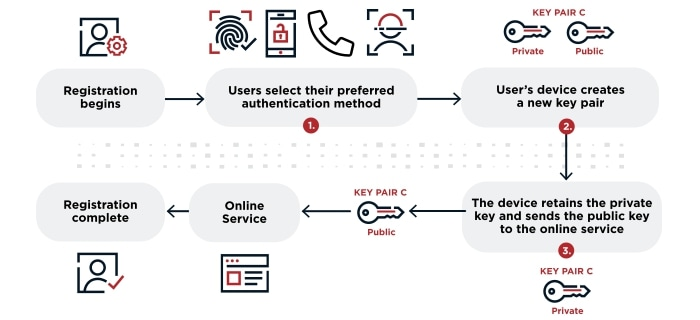
\includegraphics[width=1\textwidth]{images/7-3.jpg}
    \caption{Registrazione FIDO.}
    \label{fig:7-3}
\end{figure}

\begin{figure}
    \centering
    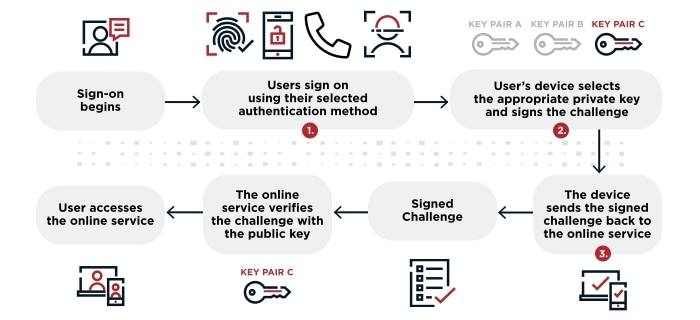
\includegraphics[width=1\textwidth]{images/7-4.jpg}
    \caption{Login FIDO.}
    \label{fig:7-4}
\end{figure}

\section{Multi-Factor Authentication}
Gli account che sono stati configurati con MFA richiedono all'utente di fornire un secondo fattore, che è qualcosa a cui solo l'utente può accedere. Generalmente questi fattori sono:
\begin{itemize}
    \item Codici inviati tramite SMS;
    \item Token da connettere fisicamente al dispositivo (anche tramite USB);
    \item Fattori biometrici;
    \item App installate su dispositivi fidati (come quelle di Microsoft e Google).
\end{itemize}

\paragraph{Ricezione delle OTP} I metodi principali per inviare/reiceve OTP sono:
\begin{itemize}
    \item SMS based: ogni volta che l'utente accede, riceve un messaggio di testo al numero di telefono registrato, che contiene una password monouso;
    \item TOTP-based: durante l'abilitazione dell'autenticazione a 2 fattori, all'utente viene chiesto di scansionare un'immagine QR utilizzando una specifica applicazione per smartphone. Tale applicazione genera quindi continuamente la One Time Password per l'utente.
\end{itemize}

\paragraph{Generazione delle OTP} Esistono più modi per generare le OPT:
\begin{itemize}
    \item HMAC-Based One Time Password Algorithm(HOTP): 
    \begin{enumerate}
        \item Il server back-end crea una chiave segreta per quel particolare utente;
        \item Il server condivide quindi la chiave segreta K con l'applicazione telefonica dell'utente;
        \item L'applicazione inizializza un contatore C;
        \item L'applicazione incrementa prima il valore del contatore di uno, quindi genera una password monouso utilizzando la chiave segreta e il contatore come segue:
        \begin{center}
            HOTP(K, C) = Tronca(HMAC-SHA1(K,C))
        \end{center}
        \item Se il valore inviato dall'applicazione telefonica corrisponde a quello generato dal server, il server incrementa il valore del contatore di uno.
    \end{enumerate}
    \item Time-based One Time Password: utilizza il tempo al posto del counter, che deve essere derivato in currentUnix time.
\end{itemize}

\section{Autenticazione FIDO}
FIDO è un protocollo di autenticazione il cui scopo è eliminare l'uso delle password, sfruttando la tecnologia della crittografia asimmetrica.

Un esempio del processo di registrazione e del processo di login sono riportate nelle immagini \ref{fig:7-3} e \ref{fig:7-4}.

